%%%%%%%%%%%%%%%%%%%%%%%%%%%%%%%%%%%%%%%%%%%%%%%%%%%%%%%%%%%%%%%%%%%%%%%%%%%%
%% Chapter 3: Methodology
%% Indian Institute of Information Technology Kalyani
%% Deep Learning-Based Polyp Detection in Colonoscopy Videos Using YOLOv8
%%%%%%%%%%%%%%%%%%%%%%%%%%%%%%%%%%%%%%%%%%%%%%%%%%%%%%%%%%%%%%%%%%%%%%%%%%%%

\chapter[Methodology]{Methodology}
\label{chp3}

\section{Introduction}
\label{chp3.1}

This chapter presents the complete methodology for developing the automated polyp detection system. The approach encompasses dataset acquisition and preprocessing, YOLOv8 architecture configuration, training strategy, inference pipeline, and evaluation framework. Figure \ref{Fig3.1} illustrates the overall system architecture.

\begin{figure}[!htb]
\begin{center}
\includegraphics[width=15cm]{Figure/chp3/system_architecture.png}
\caption{Overall system architecture: Data flow from raw dataset through preprocessing, training, inference, and evaluation}
\label{Fig3.1}
\end{center}
\end{figure}

\section{Dataset Description}
\label{chp3.2}

\subsection{Kvasir-SEG Dataset}

The Kvasir-SEG dataset \cite{jha2020kvasir} serves as the primary training and validation source. Key characteristics:

\textbf{Dataset Composition:}
\begin{itemize}
\item \textbf{Total Images}: 1,000 annotated colonoscopy frames
\item \textbf{Image Resolution}: Variable (from $332 \times 487$ to $1920 \times 1072$ pixels)
\item \textbf{Format}: JPEG images with corresponding binary masks
\item \textbf{Annotation Type}: Pixel-level segmentation masks (white polyp, black background)
\item \textbf{Source}: Real colonoscopy procedures from Vestre Viken Health Trust, Norway
\end{itemize}

\textbf{Polyp Characteristics in Dataset:}
\begin{itemize}
\item Size range: 5mm to 40mm diameter
\item Multiple morphologies: Sessile, pedunculated, flat
\item Various locations: Across different colon segments
\item Diverse appearances: Different colors, textures, lighting conditions
\end{itemize}

\textbf{Dataset Advantages:}
\begin{enumerate}
\item Public availability for reproducibility
\item High-quality expert annotations
\item Sufficient diversity for training robust models
\item Established benchmark for comparison with prior work
\item Pixel-level masks convertible to bounding boxes
\end{enumerate}

\subsection{Test Video Dataset}

For real-world validation, seven medical endoscopy videos were obtained:

\begin{table}[htb]
\centering
\caption{Test Video Dataset Characteristics}
\label{Tab3.1}
\begin{tabular}{|l|c|c|l|}
\hline
\textbf{Video Name} & \textbf{Size (MB)} & \textbf{Format} & \textbf{Polyp Type} \\
\hline
PolipoMSDz2.mpv & 7.0 & MPV & MSD Variant \\
Pediculado3.mpv & 3.8 & MPV & Pedunculated \\
Polypileocecalvalve1.mpv & 0.96 & MPV & Ileocecal Valve \\
PolipoMSDz6.mpv & - & MPV & MSD Variant \\
Pediculado5.mpv & - & MPV & Pedunculated \\
Polypvvv.mpv & - & MPV & Variant \\
Rectalcarpet1.mpv & - & MPV & Rectal Carpet \\
\hline
\end{tabular}
\end{table}

These videos provide diverse polyp presentations for comprehensive system validation.

\section{Data Preprocessing Pipeline}
\label{chp3.3}

\subsection{Segmentation Mask to Bounding Box Conversion}

The Kvasir-SEG dataset provides segmentation masks, which must be converted to YOLO bounding box format. Two conversion strategies were implemented:

\textbf{Strategy 1: Single Bounding Box (Default)}

For each mask image:
\begin{enumerate}
\item Read binary mask (0 = background, 255 = polyp)
\item Identify all polyp pixels (value = 255)
\item Compute minimum and maximum coordinates:
   \begin{align}
   x_{\min} &= \min(x \mid \text{mask}[x, y] = 255) \\
   x_{\max} &= \max(x \mid \text{mask}[x, y] = 255) \\
   y_{\min} &= \min(y \mid \text{mask}[x, y] = 255) \\
   y_{\max} &= \max(y \mid \text{mask}[x, y] = 255)
   \end{align}
\item Create single bounding box enclosing all polyp regions
\end{enumerate}

\textbf{Strategy 2: Multi-Component Detection (--multi flag)}

For polyps with disconnected regions:
\begin{enumerate}
\item Apply OpenCV connected component analysis:
   \begin{lstlisting}[language=Python]
num_labels, labels = cv2.connectedComponents(mask)
   \end{lstlisting}
\item For each connected component (excluding background):
   \begin{itemize}
   \item Extract component mask
   \item Compute bounding box coordinates
   \item Create separate YOLO label
   \end{itemize}
\item Filter small components (area $<$ threshold to remove noise)
\end{enumerate}

\textbf{YOLO Label Format Conversion:}

Convert pixel coordinates to YOLO normalized format:
\begin{align}
x_{\text{center}} &= \frac{x_{\min} + x_{\max}}{2 \cdot W} \\
y_{\text{center}} &= \frac{y_{\min} + y_{\max}}{2 \cdot H} \\
w &= \frac{x_{\max} - x_{\min}}{W} \\
h &= \frac{y_{\max} - y_{\min}}{H}
\end{align}

where $W$ and $H$ are image width and height.

Final YOLO label format per line:
\begin{verbatim}
class_id x_center y_center width height
\end{verbatim}

For polyp detection: \texttt{class\_id = 0} (single class)

Example label file content:
\begin{verbatim}
0 0.512345 0.678901 0.234567 0.345678
\end{verbatim}

\begin{figure}[!htb]
\begin{center}
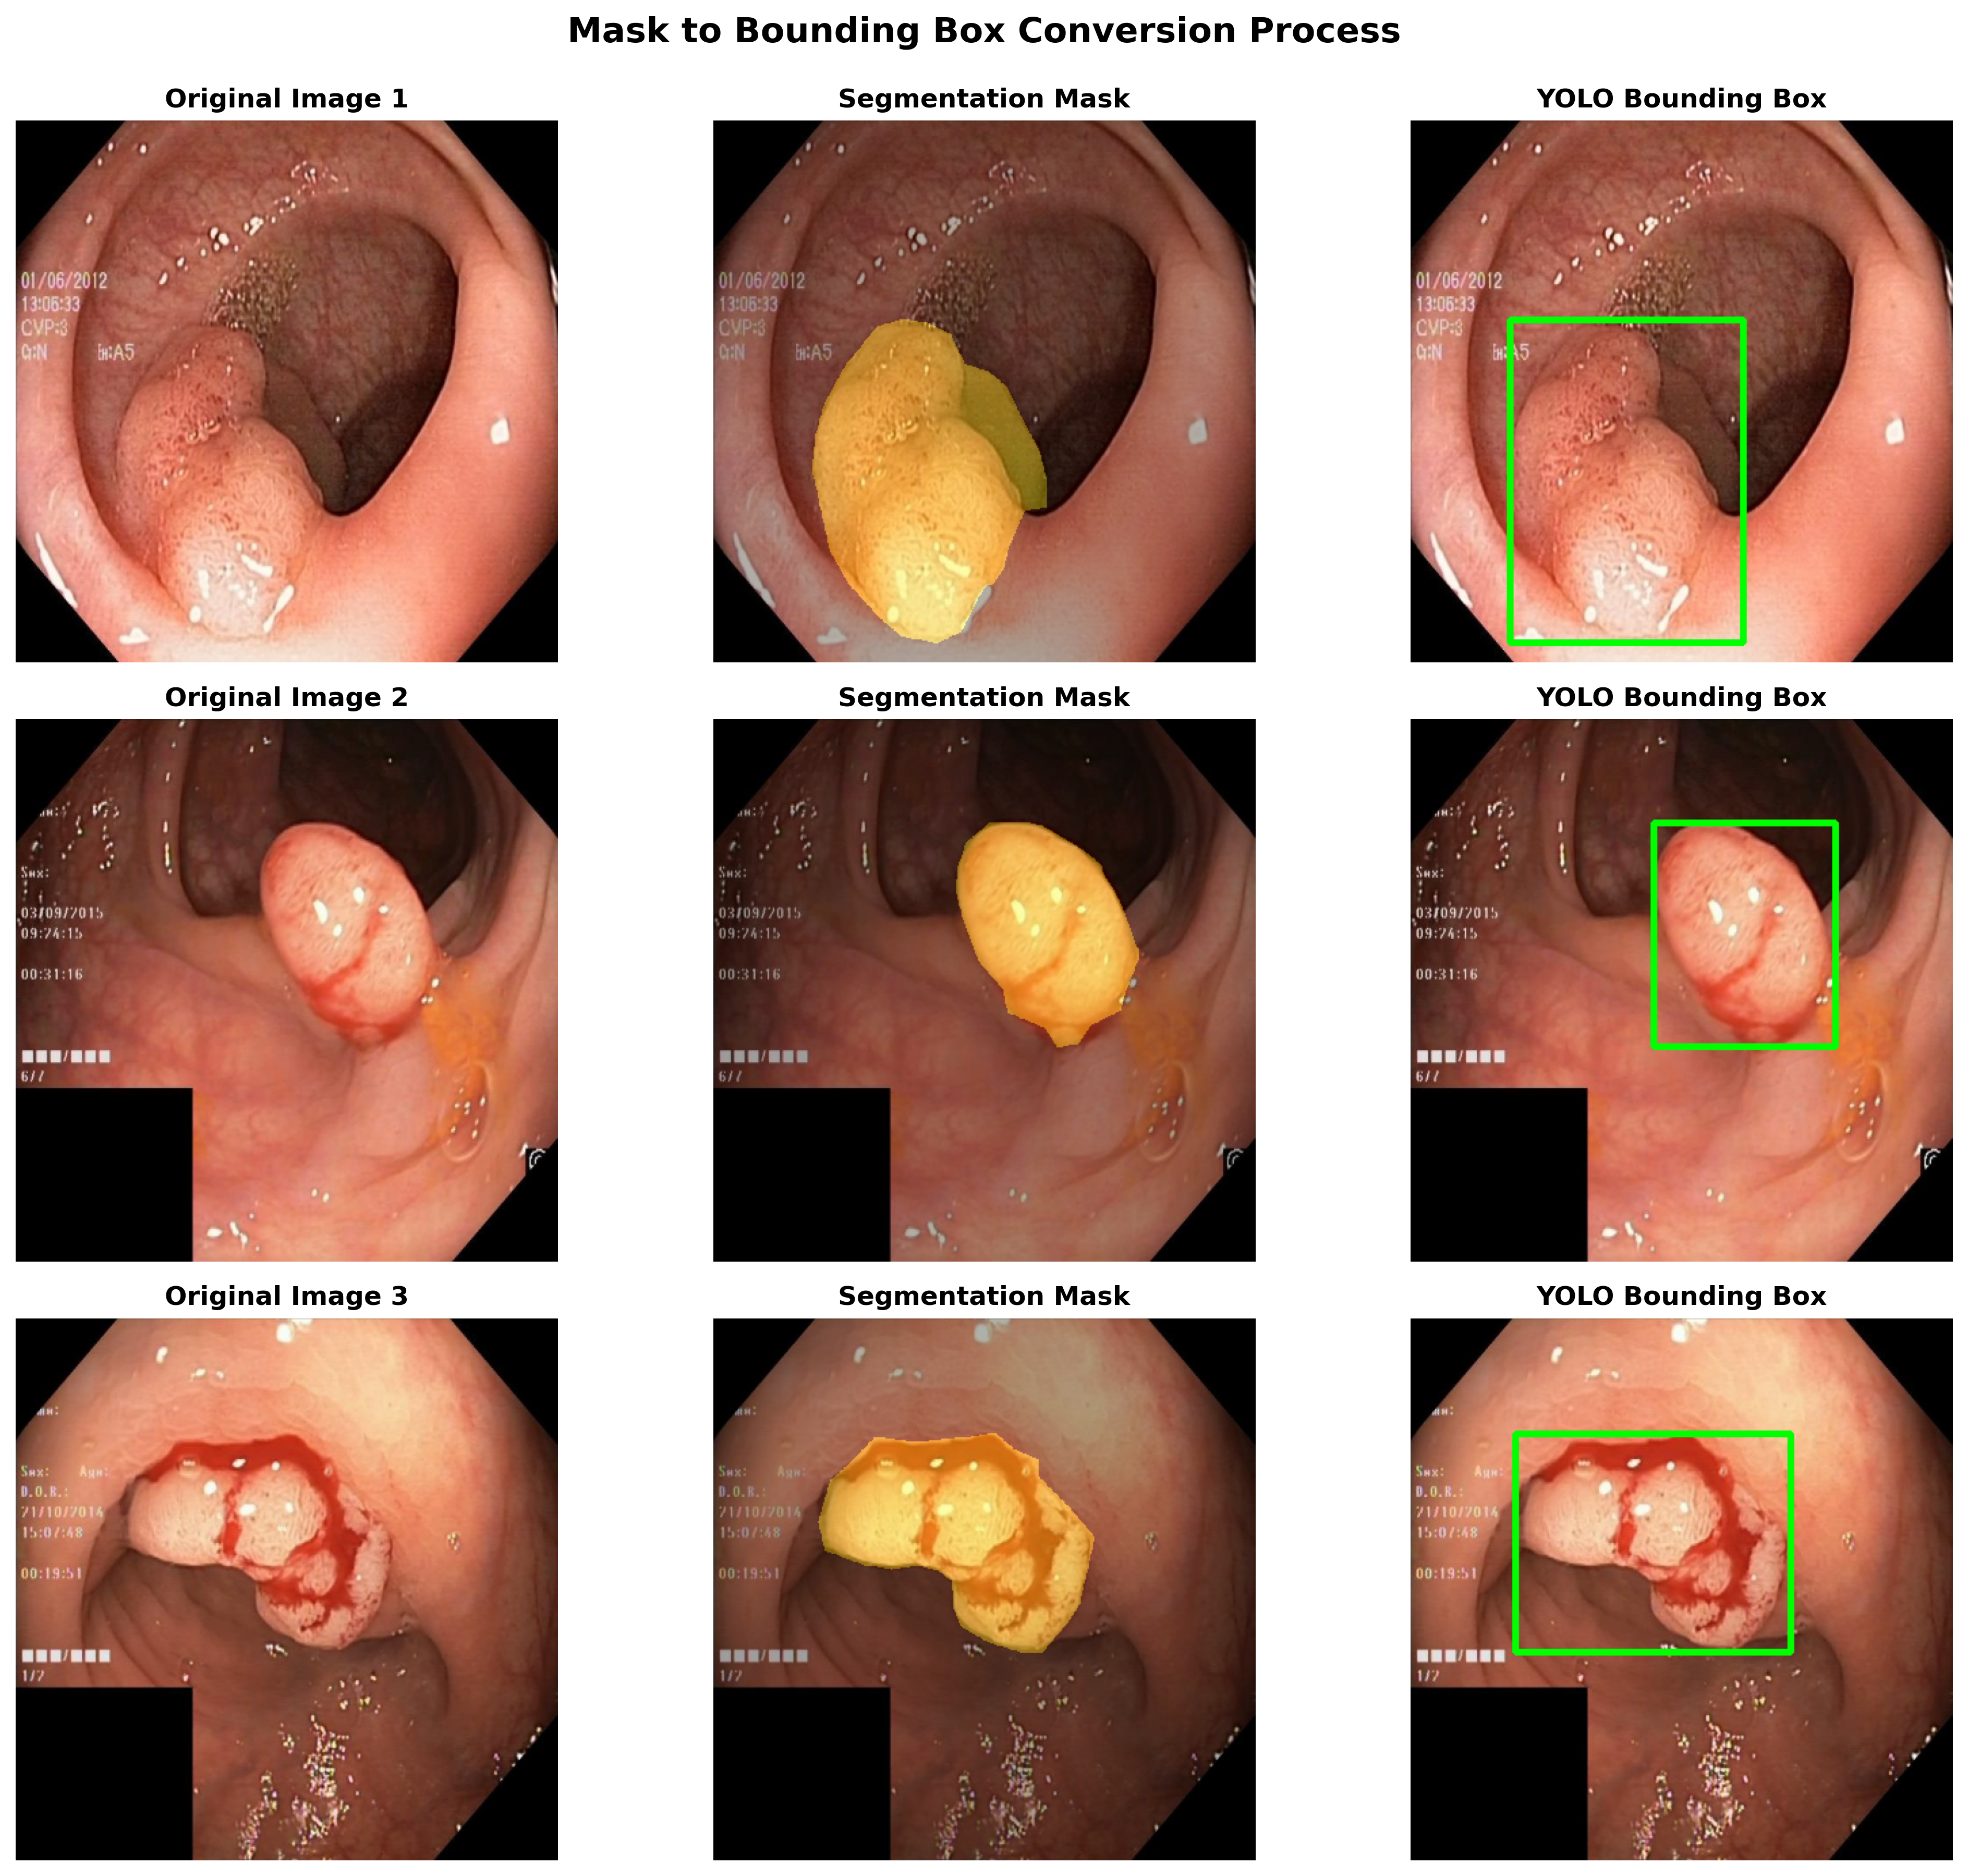
\includegraphics[width=14cm]{Figure/chp3/mask_to_bbox.png}
\caption{Mask to bounding box conversion: (a) Original image, (b) Binary segmentation mask, (c) Generated bounding box, (d) Multi-component detection}
\label{Fig3.2}
\end{center}
\end{figure}

\subsection{Train-Validation Split}

Proper data splitting ensures unbiased evaluation:

\textbf{Splitting Strategy:}
\begin{itemize}
\item \textbf{Ratio}: 80\% training, 20\% validation
\item \textbf{Method}: Random shuffling with fixed seed
\item \textbf{Seed}: 42 (for reproducibility)
\item \textbf{Result}: 800 training images, 200 validation images
\end{itemize}

\textbf{Directory Structure:}
\begin{verbatim}
data/processed/
├── images/
│   ├── train/  (800 images)
│   └── val/    (200 images)
└── labels/
    ├── train/  (800 .txt files)
    └── val/    (200 .txt files)
\end{verbatim}

\textbf{Matching Requirement:}
For each image file (e.g., \texttt{image001.jpg}), a corresponding label file (\texttt{image001.txt}) must exist with matching basename.

\subsection{Data Augmentation}

During training, YOLOv8 applies extensive augmentation:

\textbf{Geometric Augmentations:}
\begin{itemize}
\item Random horizontal flipping (p=0.5)
\item Random scaling (0.5x to 1.5x)
\item Random rotation ($\pm 10°$)
\item Random translation ($\pm 10\%$ of image size)
\end{itemize}

\textbf{Photometric Augmentations:}
\begin{itemize}
\item HSV color space perturbations
   \begin{itemize}
   \item Hue: $\pm 0.015$
   \item Saturation: $\pm 0.7$
   \item Value: $\pm 0.4$
   \end{itemize}
\item Brightness adjustment
\item Contrast modification
\end{itemize}

\textbf{Advanced Augmentations:}
\begin{itemize}
\item \textbf{Mosaic}: Combines 4 images into one (Figure \ref{Fig3.3})
\item \textbf{Mixup}: Blends two images and labels
\item \textbf{Copy-Paste}: Copies polyp instances to different backgrounds
\end{itemize}

These augmentations increase effective dataset size and improve model generalization.

\begin{figure}[!htb]
\begin{center}
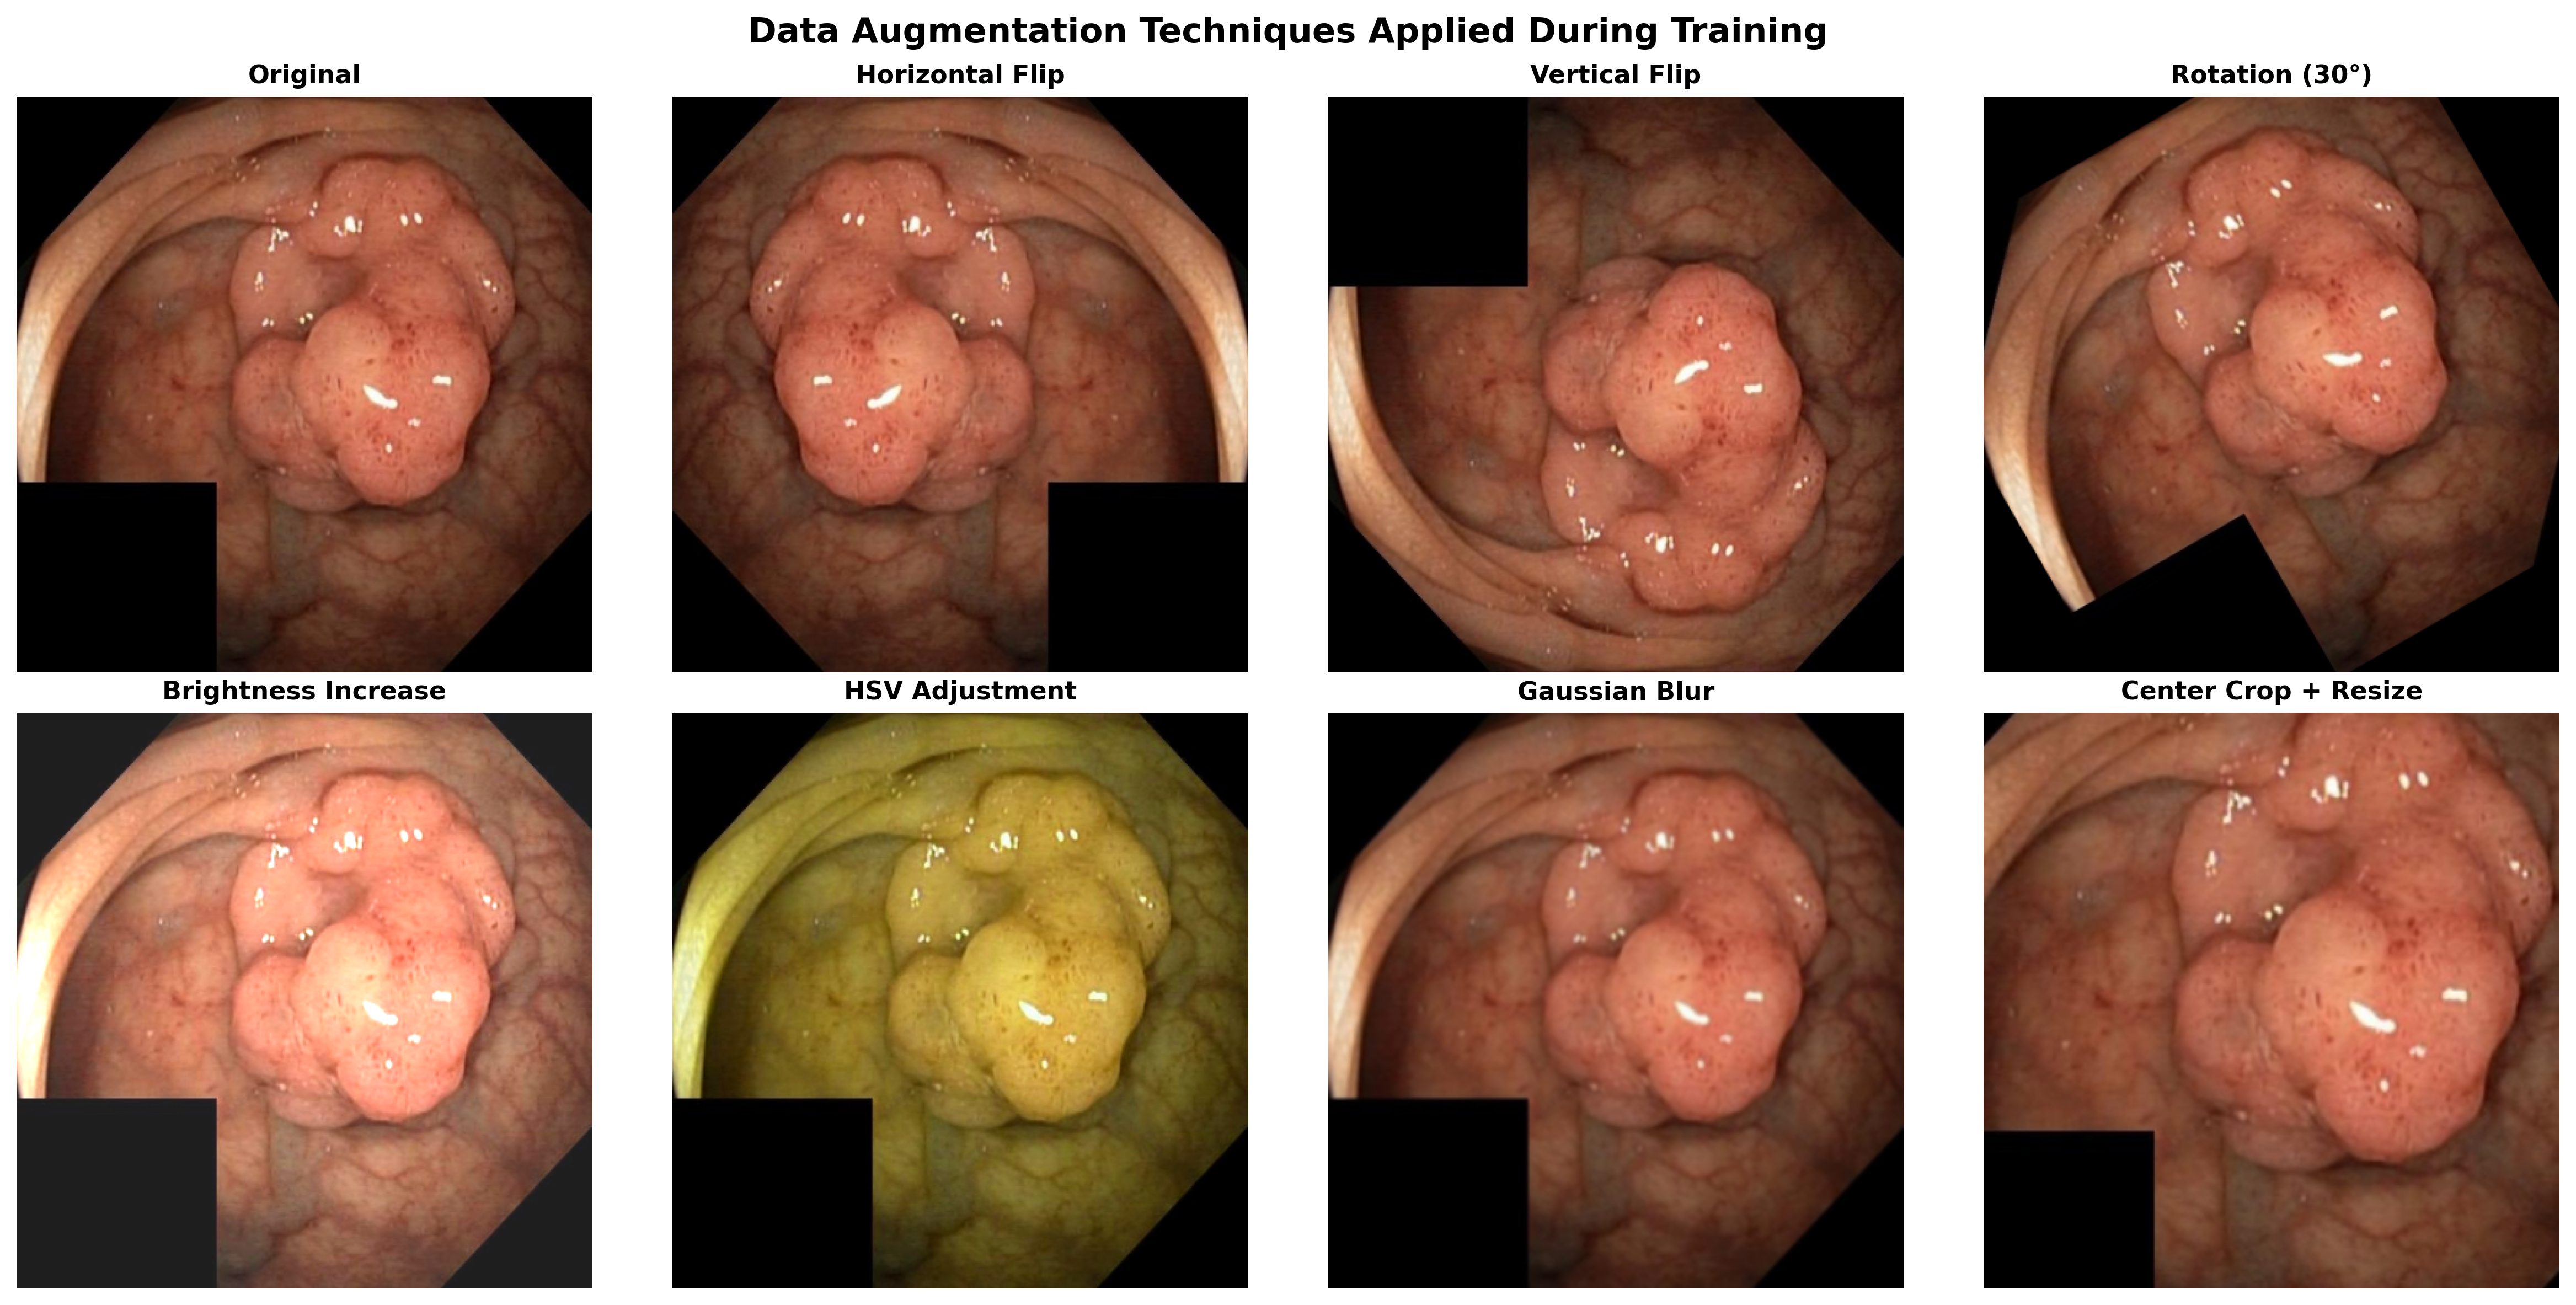
\includegraphics[width=12cm]{Figure/chp3/augmentation_examples.png}
\caption{Data augmentation examples: (a) Original, (b) Flipped, (c) Color adjusted, (d) Mosaic augmentation}
\label{Fig3.3}
\end{center}
\end{figure}

\section{YOLOv8 Architecture}
\label{chp3.4}

\subsection{Architecture Overview}

YOLOv8 introduces significant improvements over previous YOLO versions:

\textbf{Key Components:}
\begin{enumerate}
\item \textbf{Backbone}: Feature extraction network (CSPDarknet variant)
\item \textbf{Neck}: Feature pyramid network for multi-scale fusion
\item \textbf{Head}: Decoupled detection head for classification and localization
\end{enumerate}

\subsection{Backbone Network}

The backbone uses Cross Stage Partial (CSP) architecture with C2f modules:

\textbf{C2f Module (CSP Bottleneck with 2 Convolutions):}
\begin{itemize}
\item Splits input into two branches
\item Processes each through convolutional layers
\item Concatenates outputs for richer feature representation
\item Reduces computational cost while maintaining accuracy
\end{itemize}

\textbf{Backbone Architecture:}
\begin{verbatim}
Input (640×640×3)
    ↓
Conv (640×640×64)
    ↓
C2f (320×320×128)
    ↓
C2f (160×160×256)
    ↓
C2f (80×80×512)
    ↓
C2f (40×40×1024)
\end{verbatim}

\subsection{Neck - Feature Pyramid Network}

The neck performs multi-scale feature fusion:

\textbf{Top-Down Pathway:}
\begin{itemize}
\item Upsamples high-level features
\item Fuses with lower-level features via concatenation
\item Preserves semantic information from deep layers
\end{itemize}

\textbf{Bottom-Up Pathway:}
\begin{itemize}
\item Downsamples low-level features
\item Integrates with higher-level features
\item Maintains spatial precision from shallow layers
\end{itemize}

This bidirectional feature flow enables detection of polyps at multiple scales.

\subsection{Detection Head}

YOLOv8 uses a decoupled head architecture:

\textbf{Decoupled Design:}
\begin{itemize}
\item \textbf{Classification Branch}: Predicts class probabilities
\item \textbf{Regression Branch}: Predicts bounding box coordinates
\item Separate branches improve task-specific learning
\end{itemize}

\textbf{Anchor-Free Detection:}
\begin{itemize}
\item Eliminates predefined anchor boxes
\item Directly predicts box centers and dimensions
\item Better generalization to unseen object shapes
\item Particularly beneficial for variable polyp morphologies
\end{itemize}

\textbf{Output Format (per detection):}
\begin{align}
\text{Output} &= [\text{class\_prob}, x_{\text{center}}, y_{\text{center}}, w, h] \\
\text{where:} \quad &\text{class\_prob} \in [0, 1] \\
&x_{\text{center}}, y_{\text{center}} \in [0, W] \times [0, H] \\
&w, h > 0
\end{align}

\subsection{Model Variants}

YOLOv8 offers multiple model sizes trading off speed and accuracy:

\begin{table}[htb]
\centering
\caption{YOLOv8 Model Variants}
\label{Tab3.2}
\begin{tabular}{|l|c|c|c|c|}
\hline
\textbf{Model} & \textbf{Params} & \textbf{FLOPs} & \textbf{Speed (FPS)} & \textbf{mAP@50} \\
\hline
YOLOv8n (Nano) & 3.2M & 8.7G & 60-80 & High \\
YOLOv8s (Small) & 11.2M & 28.6G & 40-50 & Higher \\
YOLOv8m (Medium) & 25.9M & 78.9G & 25-30 & Higher \\
YOLOv8l (Large) & 43.7M & 165.2G & 15-20 & Highest \\
YOLOv8x (XLarge) & 68.2M & 257.8G & 10-15 & Highest \\
\hline
\end{tabular}
\end{table}

\textbf{Model Selection: YOLOv8n}

For this application, YOLOv8-nano was selected because:
\begin{itemize}
\item Real-time processing requirement (30+ FPS)
\item Limited computational resources in clinical settings
\item Sufficient accuracy for polyp detection
\item Faster training iterations during development
\item Smaller model size for deployment (6MB)
\end{itemize}

\section{Training Configuration}
\label{chp3.5}

\subsection{Training Hyperparameters}

\begin{table}[htb]
\centering
\caption{Training Hyperparameters}
\label{Tab3.3}
\begin{tabular}{|l|l|}
\hline
\textbf{Parameter} & \textbf{Value} \\
\hline
Model & YOLOv8n \\
Pretrained Weights & COCO pretrained \\
Epochs & 50 \\
Batch Size & 16 \\
Image Size & 640 $\times$ 640 \\
Learning Rate (Initial) & 0.01 \\
Learning Rate (Final) & 0.0001 \\
Optimizer & SGD (momentum=0.937) \\
Weight Decay & 0.0005 \\
Warmup Epochs & 3 \\
Loss Function & Combined (Classification + Box + DFL) \\
IoU Threshold (NMS) & 0.7 \\
Confidence Threshold & 0.25 \\
\hline
\end{tabular}
\end{table}

\subsection{Loss Function}

YOLOv8 uses a composite loss function:

\begin{equation}
\mathcal{L}_{\text{total}} = \lambda_{\text{cls}} \mathcal{L}_{\text{cls}} + \lambda_{\text{box}} \mathcal{L}_{\text{box}} + \lambda_{\text{dfl}} \mathcal{L}_{\text{dfl}}
\end{equation}

\textbf{Classification Loss (Binary Cross-Entropy):}
\begin{equation}
\mathcal{L}_{\text{cls}} = -\frac{1}{N} \sum_{i=1}^{N} [y_i \log(p_i) + (1-y_i) \log(1-p_i)]
\end{equation}
where $y_i$ is ground truth, $p_i$ is predicted probability.

\textbf{Box Regression Loss (Complete IoU):}
\begin{equation}
\mathcal{L}_{\text{box}} = 1 - \text{CIoU}(B_{\text{pred}}, B_{\text{gt}})
\end{equation}

CIoU (Complete IoU) considers:
\begin{itemize}
\item Overlap area (standard IoU)
\item Center point distance
\item Aspect ratio consistency
\end{itemize}

\textbf{Distribution Focal Loss (DFL):}
\begin{equation}
\mathcal{L}_{\text{dfl}} = -((y_+ - y) \log(\sigma_y) + (y - y_-) \log(\sigma_{y+1}))
\end{equation}

DFL enables the model to focus on ambiguous bounding box boundaries.

\textbf{Loss Weights:}
\begin{align}
\lambda_{\text{cls}} &= 0.5 \quad \text{(classification weight)} \\
\lambda_{\text{box}} &= 7.5 \quad \text{(box regression weight)} \\
\lambda_{\text{dfl}} &= 1.5 \quad \text{(distribution focal loss weight)}
\end{align}

\subsection{Learning Rate Schedule}

A cosine annealing schedule with warmup is employed:

\textbf{Warmup Phase (Epochs 1-3):}
\begin{equation}
\text{lr}(t) = \text{lr}_{\text{initial}} \cdot \frac{t}{t_{\text{warmup}}}
\end{equation}

\textbf{Cosine Annealing Phase (Epochs 4-50):}
\begin{equation}
\text{lr}(t) = \text{lr}_{\text{final}} + \frac{1}{2}(\text{lr}_{\text{initial}} - \text{lr}_{\text{final}}) \left(1 + \cos\left(\frac{t - t_{\text{warmup}}}{T - t_{\text{warmup}}} \pi\right)\right)
\end{equation}

where $T = 50$ is total epochs.

This schedule:
\begin{itemize}
\item Prevents unstable training in early epochs
\item Gradually reduces learning rate for fine-tuning
\item Helps escape local minima
\end{itemize}

\subsection{Training Environment}

\textbf{Hardware:}
\begin{itemize}
\item GPU: [Specify your GPU, e.g., NVIDIA RTX 3090]
\item RAM: [Specify, e.g., 32GB]
\item Storage: SSD for fast data loading
\end{itemize}

\textbf{Software:}
\begin{itemize}
\item Python 3.8+
\item PyTorch 2.9.1
\item CUDA 11.8
\item Ultralytics 8.3.228
\item OpenCV 4.12.0.88
\end{itemize}

\textbf{Training Duration:}
\begin{itemize}
\item Total time: ~7.15 hours for 50 epochs
\item Time per epoch: ~8.5 minutes
\item Images per second: ~60 during training
\end{itemize}

\section{Inference Pipeline}
\label{chp3.6}

\subsection{Single Image Inference}

For static image detection:

\begin{algorithm}[H]
\caption{Single Image Inference}
\label{Alg3.1}
\KwIn{Image $I$, Model $M$, Confidence threshold $\theta_c$}
\KwOut{Detected bounding boxes $B$, Confidence scores $S$}
Resize $I$ to $640 \times 640$\;
Normalize pixel values to $[0, 1]$\;
$R \leftarrow M(I)$ \tcp{Forward pass}
$B', S' \leftarrow$ Filter predictions where $s_i > \theta_c$\;
$B, S \leftarrow$ Apply Non-Maximum Suppression (NMS)\;
\Return{$B, S$}
\end{algorithm}

\subsection{Video Inference}

For colonoscopy video processing:

\begin{algorithm}[H]
\caption{Video Inference with Frame Skipping}
\label{Alg3.2}
\KwIn{Video $V$, Model $M$, Skip factor $k$, Confidence $\theta_c$}
\KwOut{Annotated video $V'$, Detection log CSV}
Initialize video reader on $V$\;
Initialize video writer for $V'$\;
Initialize CSV file with headers\;
$f \leftarrow 0$ \tcp{Frame counter}
\While{frames available}{
    Read frame $F$\;
    $f \leftarrow f + 1$\;
    \If{$f \mod k \neq 0$}{
        \textbf{continue} \tcp{Skip frame}
    }
    $B, S \leftarrow$ Infer($F$, $M$, $\theta_c$)\;
    $F' \leftarrow$ DrawBoundingBoxes($F$, $B$, $S$)\;
    Write $F'$ to $V'$\;
    \For{each detection $(b, s)$ in $(B, S)$}{
        Write $[f, \text{class}, s, b]$ to CSV\;
    }
}
Close all files\;
\Return{$V'$, CSV}
\end{algorithm}

\textbf{Frame Skipping Benefits:}
\begin{itemize}
\item Processing every $k$-th frame reduces computation
\item For $k=2$: 2x speedup, minimal accuracy loss for slow-moving videos
\item Trade-off: Speed vs. temporal resolution
\end{itemize}

\subsection{Non-Maximum Suppression}

NMS eliminates redundant overlapping detections:

\begin{algorithm}[H]
\caption{Non-Maximum Suppression}
\label{Alg3.3}
\KwIn{Boxes $B$, Scores $S$, IoU threshold $\theta_{\text{iou}}$}
\KwOut{Filtered boxes $B'$, scores $S'$}
Sort $B$, $S$ by scores in descending order\;
$B' \leftarrow \emptyset$, $S' \leftarrow \emptyset$\;
\While{$B$ not empty}{
    $b_{\max}, s_{\max} \leftarrow$ Pop highest score box\;
    $B' \leftarrow B' \cup \{b_{\max}\}$, $S' \leftarrow S' \cup \{s_{\max}\}$\;
    \For{each remaining box $b_i$ in $B$}{
        \If{IoU($b_{\max}$, $b_i$) $> \theta_{\text{iou}}$}{
            Remove $b_i$ from $B$ \tcp{Suppress overlapping box}
        }
    }
}
\Return{$B'$, $S'$}
\end{algorithm}

\section{Evaluation Framework}
\label{chp3.7}

\subsection{Validation Metrics}

The model is evaluated using standard object detection metrics:

\textbf{1. Precision-Recall Curve:}

Precision and recall computed at various confidence thresholds:
\begin{align}
\text{Precision}(\theta) &= \frac{\text{TP}(\theta)}{\text{TP}(\theta) + \text{FP}(\theta)} \\
\text{Recall}(\theta) &= \frac{\text{TP}(\theta)}{\text{TP}(\theta) + \text{FN}(\theta)}
\end{align}

\textbf{2. Average Precision (AP):}

Area under precision-recall curve:
\begin{equation}
\text{AP} = \int_0^1 P(R) \, dR \approx \sum_{i=1}^{N} P_i (R_i - R_{i-1})
\end{equation}

\textbf{3. mean Average Precision (mAP):}

\begin{itemize}
\item \textbf{mAP@50}: AP at IoU threshold 0.5
\item \textbf{mAP@50-95}: Average AP across IoU $\in \{0.50, 0.55, ..., 0.95\}$:
\begin{equation}
\text{mAP@50-95} = \frac{1}{10} \sum_{i=0}^{9} \text{AP}(0.50 + 0.05i)
\end{equation}
\end{itemize}

\textbf{4. F1-Score:}

Harmonic mean of precision and recall:
\begin{equation}
\text{F1} = \frac{2 \cdot \text{Precision} \cdot \text{Recall}}{\text{Precision} + \text{Recall}}
\end{equation}

\subsection{Evaluation Protocol}

\textbf{Validation Set Evaluation:}
\begin{enumerate}
\item Run inference on all 200 validation images
\item Compare predictions with ground truth labels
\item Compute metrics at IoU thresholds 0.5 to 0.95
\item Generate precision-recall curves
\item Calculate mAP@50 and mAP@50-95
\end{enumerate}

\textbf{Video Test Evaluation:}
\begin{enumerate}
\item Process each test video frame-by-frame
\item Log all detections with confidence scores
\item Generate annotated video with bounding boxes
\item Analyze detection statistics:
   \begin{itemize}
   \item Total detections
   \item Confidence score distribution
   \item Detection rate (frames with polyps / total frames)
   \item Maximum/minimum/average confidence
   \end{itemize}
\end{enumerate}

\section{Summary}
\label{chp3.8}

This chapter presented the comprehensive methodology for the polyp detection system. The Kvasir-SEG dataset with 1,000 annotated images provides the training foundation, supplemented by seven real medical videos for validation. The data preprocessing pipeline converts segmentation masks to YOLO format using both single and multi-component strategies.

The YOLOv8-nano architecture was selected for its optimal speed-accuracy balance, featuring a CSP backbone, feature pyramid neck, and decoupled anchor-free detection head. Training employs 50 epochs with extensive augmentation (mosaic, mixup, color adjustments) using a composite loss function and cosine annealing learning rate schedule.

The inference pipeline supports both single images and videos with frame skipping optimization. Evaluation uses standard object detection metrics (mAP@50, mAP@50-95, precision, recall) on the validation set, complemented by comprehensive video analysis with detection logging and visual annotation. This robust methodology ensures both high performance and clinical applicability.
